% Original vector reconstruction of source Fig.81.2, PDF332 / printed320.
% Solid-line arrows are quark charge arrows. Parallel wavy-line arrows
% specify gluon momenta. All external momenta are assigned outward.
% Internal p5 runs down the first graph; internal k5 runs left in the second.
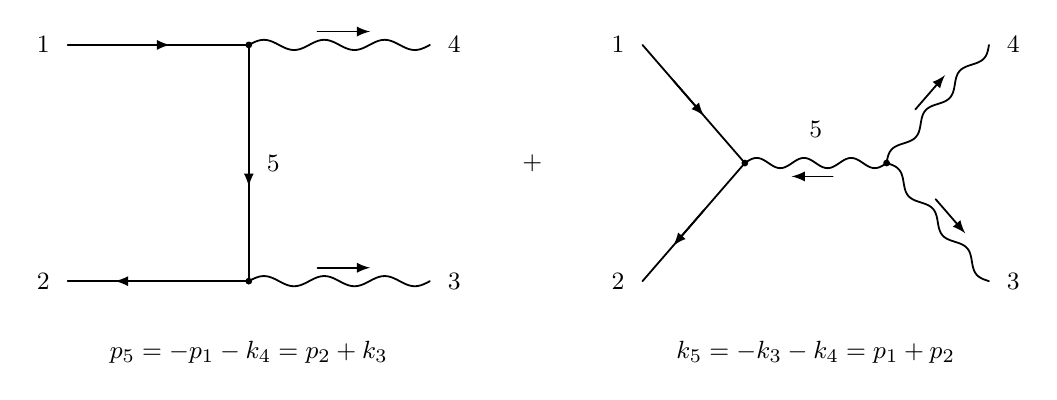
\begin{tikzpicture}[x=1mm,y=1mm,line width=.65pt,>=latex,
  line cap=round,line join=round,font=\fontsize{9.5}{11.5}\selectfont]
  \def\sW#1#2#3{%
    \begin{scope}[shift={#1},rotate=#2]
      \draw plot[domain=0:1,samples=61]
        ({#3*\x},{.65*sin(1080*\x)});
      \draw[->] ({.38*#3},1.7)--({.67*#3},1.7);
    \end{scope}}
  \begin{scope}[shift={(29,0)}]
    \draw (-23,15)--(0,15)--(0,-15)--(-23,-15);
    \draw[->] (-17,15)--(-10,15);
    \draw[->] (0,5)--(0,-3);
    \draw[->] (-10,-15)--(-17,-15);
    \sW{(0,15)}{0}{23}
    \sW{(0,-15)}{0}{23}
    \fill (0,15) circle[radius=.43mm];
    \fill (0,-15) circle[radius=.43mm];
    \node[left] at (-24,15) {$1$};
    \node[left] at (-24,-15) {$2$};
    \node[right] at (24,-15) {$3$};
    \node[right] at (24,15) {$4$};
    \node[right] at (1,0) {$5$};
    \node at (0,-24) {$p_5=-p_1-k_4=p_2+k_3$};
  \end{scope}
  \node at (65,0) {$+$};
  \begin{scope}[shift={(101,0)}]
    \draw (-22,15)--(-9,0)--(-22,-15);
    \draw[->] (-18.1,10.5)--(-14.2,6);
    \draw[->] (-14.2,-6)--(-18.1,-10.5);
    \sW{(9,0)}{180}{18}
    \sW{(9,0)}{49.085617}{19.849433}
    \sW{(9,0)}{-49.085617}{19.849433}
    \fill (-9,0) circle[radius=.43mm];
    \fill (9,0) circle[radius=.43mm];
    \node[left] at (-23,15) {$1$};
    \node[left] at (-23,-15) {$2$};
    \node[right] at (23,-15) {$3$};
    \node[right] at (23,15) {$4$};
    \node[above] at (0,2) {$5$};
    \node at (0,-24) {$k_5=-k_3-k_4=p_1+p_2$};
  \end{scope}
\end{tikzpicture}

